\documentclass[tikz]{standalone}

\usepackage{amsfonts}
\usepackage{amsmath}
\usepackage{braket}

\usepackage{tikz}
\usetikzlibrary{calc, decorations, positioning}

% load TikZ grafic definitions
%\input{gfx_TikZ}

% main document
\begin{document}

	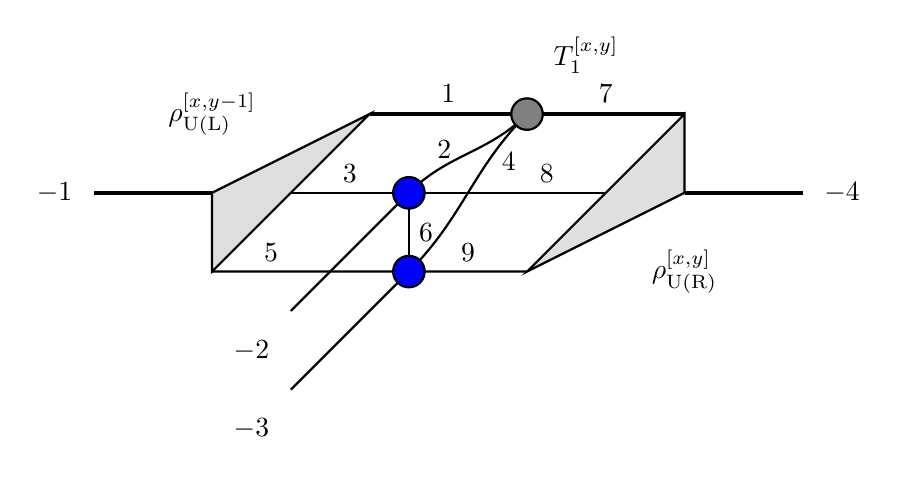
\begin{tikzpicture}[]

		% contant definitions
		\def\tensorSize{0.2}

		% tensor network contraction
		\begin{scope}[shift = {(+2.0, -0.5)}]

			% iPEPS network coordinates
			\coordinate (PN) at (+0.0, +0.5);
			\coordinate (PC) at (+0.0, -0.5);

			% CTMRG network coordinates
			\coordinate (C1) at (-0.5, +1.5);
			\coordinate (T1) at (+1.5, +1.5);
			\coordinate (C2) at (+3.5, +1.5);
			\coordinate (T2) at (+2.0, +0.0);
			\coordinate (C3) at (+0.5, -1.5);
			\coordinate (T3) at (-1.5, -1.5);
			\coordinate (C4) at (-3.5, -1.5);
			\coordinate (T4) at (-2.0, -0.0);

			% projector P_{UL}
			\begin{scope}[shift = {(-2.50, +0.50)}]
				\coordinate (PLL) at (+0.00, +0.00);
				\coordinate (PLU) at (+2.00, +1.00);
				\coordinate (PLM) at (+1.00, +0.00);
				\coordinate (PLD) at (+0.00, -1.00);
				\node[] at (+0.00, +1.00) {$\rho_\text{U(L)}^{[x, y - 1]}$};
			\end{scope}

			% projector P_{UR}
			\begin{scope}[shift = {(+3.50, +0.50)}]
				\coordinate (PRU) at (+0.00, +1.00);
				\coordinate (PRM) at (-1.00, -0.00);
				\coordinate (PRD) at (-2.00, -1.00);
				\coordinate (PRR) at (+0.00, +0.00);
				\node[] at (-0.00, -1.00) {$\rho_\text{U(R)}^{[x, y]}$};
			\end{scope}

			% tensor labels
			\node at ($(T1) + (+0.75, +0.75)$) {$T_1^{[x, y]}$};
			
			% external links
			\draw[thick] (PN) to ($(PN) + (-1.50, -1.50)$) node at ($(PN) + (-2.00, -2.00)$) {$-2$};
			\draw[thick] (PC) to ($(PC) + (-1.50, -1.50)$) node at ($(PC) + (-2.00, -2.00)$) {$-3$};
			\draw[ultra thick] (PLL) to ($(PLL) + (-1.50, -0.00)$) node at ($(PLL) + (-2.00, -0.00)$) {$-1$};
			\draw[ultra thick] (PRR) to ($(PRR) + (+1.50, +0.00)$) node at ($(PRR) + (+2.00, +0.00)$) {$-4$};
			
			% projectors
			\draw[thick, fill = gray!25] (PLL) to (PLU) to (PLD) -- cycle;
			\draw[thick, fill = gray!25] (PRR) to (PRU) to (PRD) -- cycle;

			% internal links
			\draw[ultra thick] (T1) -- (PLU) node[above] at ($(T1)!0.5!(PLU)$) {$1$};
			\draw[ultra thick] (T1) -- (PRU) node[above] at ($(T1)!0.5!(PRU)$) {$7$};
			\draw[thick] (PN) to [out = 180, in = 0] (PLM) node[above] at ($(PN)!0.5!(PLM)$) {$3$};
			\draw[thick] (PRM) to [out = 180, in = 0] (PN) node[above] at ($(PRM)!0.3!(PN)$) {$8$};
			\draw[thick] (PC) to [out = 180, in = 0] (PLD) node[above] at ($(PC)!0.7!(PLD)$) {$5$};
			\draw[thick] (PRD) to [out = 180, in = 0] (PC) node[above] at ($(PRD)!0.5!(PC)$) {$9$};
			\draw[thick] (T1) to [out = 225, in = 45] (PC) node[right] at ($(T1)!0.3!(PC)$) {$4$};
			\draw[thick] (T1) to [out = 225, in = 45] (PN) node[above] at ($(T1)!0.7!(PN)$) {$2$};
			\draw[thick] (PN) -- (PC) node [midway, right] {$6$};

			% CTMRG tensors
			\foreach \tensor in {T1} {
				\draw[thick,black,fill = gray] (\tensor) circle (\tensorSize);
			}

			% iPEPS tensors
			\foreach \tensor in {PN, PC} {
				\draw[thick,black,fill = blue] (\tensor) circle (\tensorSize);
			}
			
		\end{scope}

	\end{tikzpicture}

\end{document}

%%% Local Variables:
%%% mode: latex
%%% TeX-master: t
%%% End:
